\subsection{Tarefa 1}

\begin{comandoquestao}
   Nesta tarefa, você explorará o impacto de diferentes funções de ativação no desempenho da rede neural. A função de ativação controla como os neurônios transformam os dados de entrada, e diferentes funções podem influenciar a capacidade de aprendizado da rede.
\end{comandoquestao}

A rede neural dada como exemplo utiliza a função Gelu como função de ativação nas camadas intermediárias. Vericamos o comportamento do erro de treinamento em relação ao número de épocas de treinamento (figura \ref{tarefa01:gelu:treinamento}), bem como a comparação dos dados previstos pela rede dados em relação aos dados de treinamento na figura \ref{tarefa01:gelu:predicoes}.

\begin{figure}[htb]
	\label{teste}
	\centering
	\begin{minipage}{0.45\textwidth}
	\centering
	\caption{Gelu: Treinamento} \label{tarefa01:gelu:treinamento}
	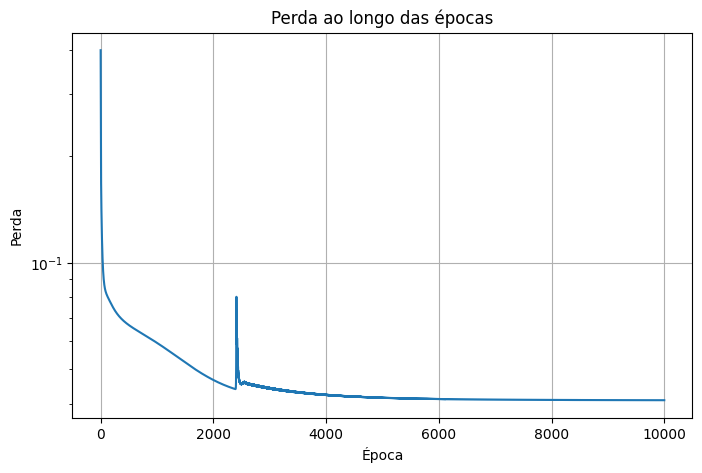
\includegraphics[width=\textwidth]{./0803_imgs/png-241111-212601400-7995113924505873963.png}
	%\legend{Fonte: Gerado peloComando da atividade}
	\end{minipage}
	\hfill
	\begin{minipage}{0.45\textwidth}
	\centering
	\caption{Gelu: predições} \label{tarefa01:gelu:predicoes}
	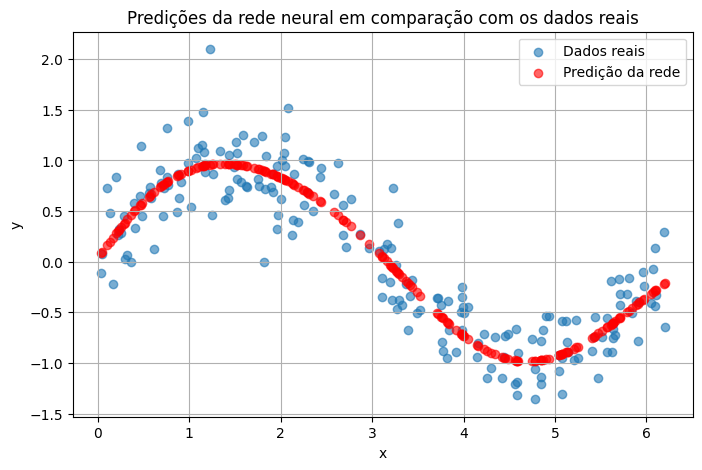
\includegraphics[width=\textwidth]{./0803_imgs/png-241111-212606975-12044568718402292765.png}
	%\legend{Fonte: \citeonline[p. 24]{araujo2012}}
	\end{minipage}
\end{figure}

Para a presente tarefa modificamos a função de ativação das camadas intermediárias para sigmóide, obtendo os resultados mostrados nas figuras


\begin{figure}[htb]
	\label{teste}
	\centering
	\begin{minipage}{0.45\textwidth}
	\centering
	\caption{Gelu: Treinamento} \label{tarefa01:gelu:treinamento}
	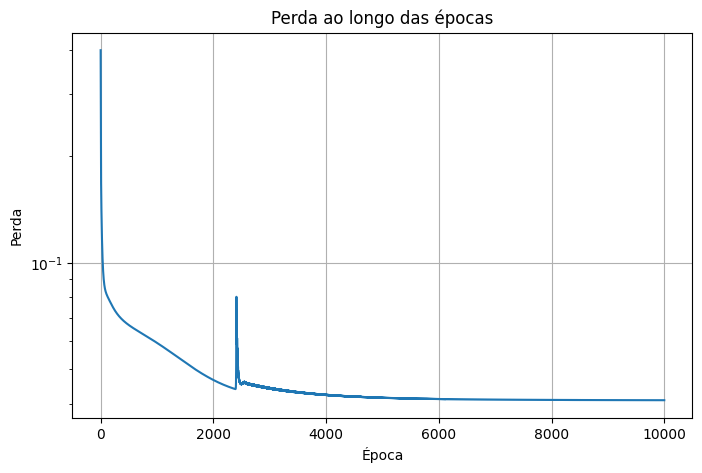
\includegraphics[width=\textwidth]{./0803_imgs/png-241111-212601400-7995113924505873963.png}
	%\legend{Fonte: Gerado peloComando da atividade}
	\end{minipage}
	\hfill
	\begin{minipage}{0.45\textwidth}
	\centering
	\caption{Gelu: predições} \label{tarefa01:gelu:predicoes}
	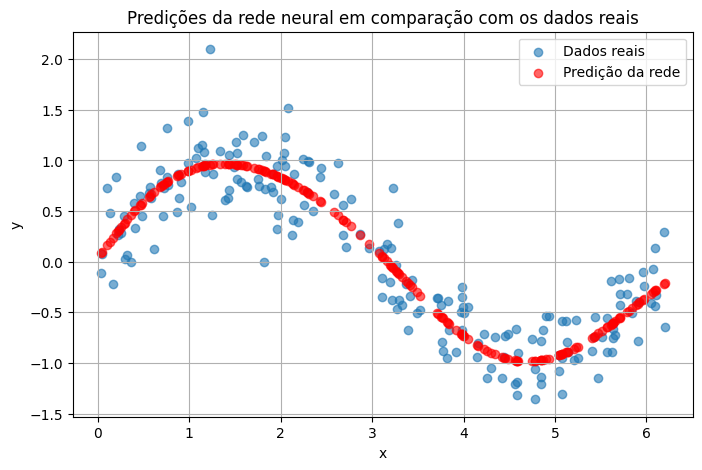
\includegraphics[width=\textwidth]{./0803_imgs/png-241111-212606975-12044568718402292765.png}
	%\legend{Fonte: \citeonline[p. 24]{araujo2012}}
	\end{minipage}
\end{figure}
